%%%%%%%%%%%%%%%%%%%%%%%%%%%%%%%%%%%%%%%%%
% Journal Article
% LaTeX Template
% Version 1.4 (15/5/16)
%
% This template has been downloaded from:
% http://www.LaTeXTemplates.com
%
% Original author:
% Frits Wenneker (http://www.howtotex.com) with extensive modifications by
% Vel (vel@LaTeXTemplates.com)
%
% License:
% CC BY-NC-SA 3.0 (http://creativecommons.org/licenses/by-nc-sa/3.0/)
%
%%%%%%%%%%%%%%%%%%%%%%%%%%%%%%%%%%%%%%%%%

%----------------------------------------------------------------------------------------
%	PACKAGES AND OTHER DOCUMENT CONFIGURATIONS
%----------------------------------------------------------------------------------------

\documentclass[twoside,twocolumn]{article}

\usepackage{blindtext} % Package to generate dummy text throughout this template 

\usepackage[sc]{mathpazo} % Use the Palatino font
\usepackage[T1]{fontenc} % Use 8-bit encoding that has 256 glyphs
\linespread{1.05} % Line spacing - Palatino needs more space between lines
\usepackage{microtype} % Slightly tweak font spacing for aesthetics

\usepackage[english]{babel} % Language hyphenation and typographical rules

\usepackage[hmarginratio=1:1,top=32mm,columnsep=20pt]{geometry} % Document margins
\usepackage[hang, small,labelfont=bf,up,textfont=it,up]{caption} % Custom captions under/above floats in tables or figures
\usepackage{booktabs} % Horizontal rules in tables

\usepackage{lettrine} % The lettrine is the first enlarged letter at the beginning of the text

\usepackage{enumitem} % Customized lists
\setlist[itemize]{noitemsep} % Make itemize lists more compact

\usepackage{abstract} % Allows abstract customization
\renewcommand{\abstractnamefont}{\normalfont\bfseries} % Set the "Abstract" text to bold
\renewcommand{\abstracttextfont}{\normalfont\small\itshape} % Set the abstract itself to small italic text

\usepackage{titlesec} % Allows customization of titles
\renewcommand\thesection{\Roman{section}} % Roman numerals for the sections
\renewcommand\thesubsection{\roman{subsection}} % roman numerals for subsections
\titleformat{\section}[block]{\large\scshape\centering}{\thesection.}{1em}{} % Change the look of the section titles
\titleformat{\subsection}[block]{\large}{\thesubsection.}{1em}{} % Change the look of the section titles

\usepackage{fancyhdr} % Headers and footers
\pagestyle{fancy} % All pages have headers and footers
\fancyhead{} % Blank out the default header
\fancyhead[C]{Indirect Reciprocity $\bullet$ Nov 2018} % Custom header text
\fancyfoot{} % Blank out the default footer
\fancyfoot[RO,LE]{\thepage} % Custom footer text

\usepackage{titling} % Customizing the title section

\usepackage{hyperref} % For hyperlinks in the PDF

\usepackage{graphicx}
\usepackage{booktabs}
\usepackage{multirow}
\usepackage{framed}
\usepackage{caption}

%----------------------------------------------------------------------------------------
%	TITLE SECTION
%----------------------------------------------------------------------------------------

\setlength{\droptitle}{-4\baselineskip} % Move the title up

\pretitle{\begin{center}\Huge\bfseries} % Article title formatting
\posttitle{\end{center}} % Article title closing formatting
\title{Report on indirect reciprocity, strategies for agents and the development of a concrete model to implement} % Article title
\author{%
\textsc{James King} \\% Your name
\normalsize Supervisor: Kostas Stathis \\ % Your supervisor
}
\date{October 2018} % Leave empty to omit a date
\renewcommand{\maketitlehookd}{%
\begin{abstract}
\noindent Indirect reciprocity is a mechanism that uses reciprocation theory to aid in the evolution of cooperation. Cooperation being an action taken by an individual that benefits another individual but at a cost to itself. Indirect reciprocity is a promising motivator for cooperation in societies with agents of higher intelligence levels and of greater sizes, such as human societies or even multi-agent systems. I plan to implement the mechanism programmatically, but there are many models and many possible additions to these models. In this report I will explore past approaches to indirect reciprocity, comparing and contrasting the variations proposed. The outcome of this exploration of approaches will be a concrete model to implement in this project.
\end{abstract}
}

%----------------------------------------------------------------------------------------

\begin{document}

% Milestone: Report on indirect reciprocity, strategies for agents and the development of a concrete model to implement
% Report on past work on indirect reciprocity including the strategies agents have employed playing this game.
% From this collated work I shall define a model which I am to implement and a number of key strategies to implement as well.
% Link to goal: This is a part of my exploration of the mechanisms that aid in the evolution of cooperation and will help provide a model to implement in system for running indirect reciprocity tournaments across the Prolog service and environment.



% Print the title
\maketitle

%----------------------------------------------------------------------------------------
%	ARTICLE CONTENTS
%----------------------------------------------------------------------------------------

\section{Introduction}
The evolution and preservation of cooperation has been a puzzle for evolutionary theorists for a long time. Many different approaches have been taken to give an explanation to cooperative phenomena, especially from the field of game theory. Often these approaches have come from the idea of reciprocity, where agents can grow mutually beneficial relationships through repeated interactions. The most popular mechanism of this being direct reciprocity where interactions are repeated between the same two individuals, and thus they may reciprocate directly with each other.\\
There is another game-theoretic mechanism known as indirect reciprocity, which works on the idea that nice agents will help those who help each other - "if I scratch your back, others will hopefully scratch mine" displayed graphically in figure~\ref{fig:indir_rec}. This means learning information about another player does not require direct interaction. A number of models have been proposed to run indirect reciprocity. It is these models I shall be describing and reviewing, before using them to formulate my own to implement in my project.
\begin{figure}
	\begin{center}
	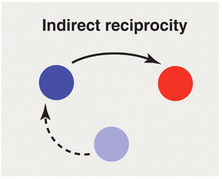
\includegraphics[width=0.3\textwidth]{Indirect_rec.png}
	\caption{The main idea of indirect reciprocity from Nowak~\cite{five_rules_coop}}
	\label{fig:indir_rec}
	\end{center}
\end{figure}


%------------------------------------------------

\section{Review of Past Work}
\subsection{Nowak, Sigmund and Image Scoring}
Nowak and Sigmund's model has a population structure of just one population of players per generation, the first generation of players are chosen at the start of an indirect reciprocity tournament~\cite{evol_indirect_image}. A population then reproduces into the next generation of players (more on reproduction further down). From the population of a generation a set of pairs of players are chosen at random to interact. A pair is made up of a donor and recipient. The donor can choose to cooperate at a cost c, from this the recipient receives b points (b>c), or defect at no cost to the donor's fitness but the recipient also receives no points.\\
The model utilizes the idea of image scoring. An image score is comparable to the idea of a player's reputation. A player's image score increases to those who see them cooperate and decreases to those who see them defect. The actual image score is an integer, bounded between -5 and 5. One key part of the model is where these image scores are held.\\
In the first formulation of this all image scores are public, but later on, it is suggested that this model is unlikely to hold true in real life as individual's views on other individuals' reputations tend to differ. As an alternative, the idea of onlookers is suggested, where a set of onlookers are chosen from the generation for each interaction. In both models, image scores are increased by one for a cooperation as a donor or decreased by one for a defection as a donor, though in the second model only the onlookers, recipient and donor can add this to their image score for the donor. The use of onlookers does make cooperation harder to establish, as it is dependent on whether a player knows an accurate image score of the recipient.\\
The points accrued through interactions gives the fitness score of each player. The amount a player reproduces into the next generation is dependent on the fitness score. Mutation is also an option in this model, this phenomenon is when a player reproduces at random their offspring can be a different strategy. Mutation can lead to loops where defectors are invaded by discriminators and then discriminators are undermined by cooperators - allowing defectors to take hold again.\\
The two simplest strategies are pure defection and pure cooperation. A key strategy for the evolution of cooperation is the discriminator strategy as illustrated in figure~\ref{fig:image_discriminator}. In fact, there is a baseline number of discriminators required for cooperation to evolve. This strategy is given a number k, if the image score of a player is greater than or equal to k a discriminator will cooperate with them. More interesting strategies take into account their own image score or theirs and the recipient's image score, these can aid in the evolution of cooperation too. In the absence of information on other players, these strategies can believe other players to have an image score of k with a certain probability.\\
The model is known to be dependent on the probability of knowing the image of another player. Cooperation can only be stable if $q > c/b$, q being the probability of knowing the image, c being the cost and b being the benefit.\\
Leimar and Hammerstein recognised the problems of genetic drift in this model~\cite{leimarhammer}. Genetic drift being "a situation in which the frequency of a particular gene in a small population of living things changes without a known cause"~\cite{genetic_drift}. Adopting an island population model to restrict genetic drift. Rather than one single population group, in the island population model, the group is divided up into g amount of groups each with population n. This model also uses a different reproductive strategy where relative reproductive success locally is calculated as a normalisation of the sum of the fitness of all strategies within the same group. For global expected reproductive success sum each strategy and normalize over the whole population. A new individual is then locally derived with probability p or globally derived with probability 1-p. The strategy for the individual produced is randomly generated with a distribution corresponding to the local or global reproductive success.
\begin{figure}
	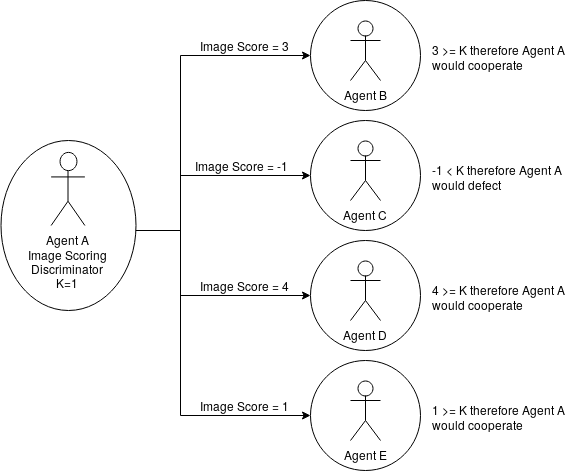
\includegraphics[width=0.5\textwidth]{Image_Scoring.png}
	\caption{How an image scoring discriminator strategy acts}
	\label{fig:image_discriminator}
\end{figure}

\subsection{Standing Strategy}
The standing strategy was suggested by both Leimar and Hammerstein~\cite{leimarhammer} and Roberts~\cite{evoldirindir} to be superior to image scoring. Their models used the island population structure given above. Leimar and Hammerstein replaced image scoring with the standing strategy whereas Roberts mixed direct and indirect reciprocity (with both image scoring and the standing strategy).\\
The standing strategy as described by Milinski \textit{et al.}~\cite{imagevsstanding} is that players should not just aim for a good fitness, but also good standing. Everyone starts on a good standing, but if a player is a donor to a good standing recipient and does not cooperate with them the donor loses their good standing.\\
The idea of this is that committing to bad actions against good individual is immoral, but it is not necessarily true that committing to good actions towards bad individual is moral and according to most game-theoretic models it does not produce stable cooperative society.\\
This is seen as a benefit over image scoring as with image scoring it is not always in a players interest to punish those with a low image score, as they lose reputation themselves and in turn reduces the likelihood of them being the recipient of a cooperation. Whereas reputation is only lost in the standing strategy if the recipient is not of a good standing.

\subsection{Mixed Reciprocity Models}
Gilbert Roberts puts forward mixed direct and indirect reciprocity models~\cite{evoldirindir} using image scoring in one model similar to Nowak and Sigmund~\cite{evol_indirect_image} and standing strategy. Both models use the island and reproductive systems Leimar and Hammerstein~\cite{leimarhammer} utilized. Roberts put forward this notion due to his perception that indirect reciprocity alone is not a generalisable concept due to the close-knit nature of many societies.\\
Decisions can be made by agents in Roberts' model on the basis of either a reputation or an experience score. Reputation scores use image scoring in one model, differing from Nowak and Sigmund's as the score is within the range -1 to 1, initially at 0, decreasing by one for a defection and increasing by 1 for a cooperation. The standing strategy version assigns a -1 to a player when they defect against an individual or 1 to a player for anything else.\\
Experience scores are analogous to direct reciprocity for Roberts. When using image scoring, the experience scores between 2 players are initially 0 and go to -1 if they have defected or 1 if they have cooperated in the previous interaction. For standing strategy -1 is assigned only if the players has defected with a partner that has an experience score of 0 or 1 with them.\\
As you can see experience scores only reflect the previous interaction between the two individuals. This is a clear limitation as the model is seeking to describe a society made up of agents that have a higher intelligence.\\
Interestingly Roberts also considers the case where an agent has no resources to cooperate and thus must defect.\\
Steve Phelps~\cite{phelps_game_theoretic_analysis} also recognises the same issue with indirect reciprocity as Gilbert Roberts - namely that remeeting in groups is likely, especially in smaller groups according to Phelps. Due to this Phelps suggests a mixed framework, to test how group sizes affect the use of direct or indirect reciprocity by agents.
 
\subsection{Gossip and Onlookers}
It is recognised by Nowak and Sigmund~\cite{evol_indirect_image} that it is unrealistic to expect all players to have directly observed a given interaction. Yet their answer - onlookers - hampers the evolution of cooperation, which relies on the probability that a player knows the image score of another player.\\
Sommerfeld \textit{et al.} highlighted the importance of communication to the management of reputations. Gossip is a type of communication that is key part of societal mechanics, the structure of which is highlighted in figure~\ref{fig:gossip_and_onlookers}. The findings of their experiment were that gossip needs to accurately reflect the interaction and the recipient of the gossip needs to correctly acted upon for gossip to be an adequate replacement for direct observation.
\begin{figure}
	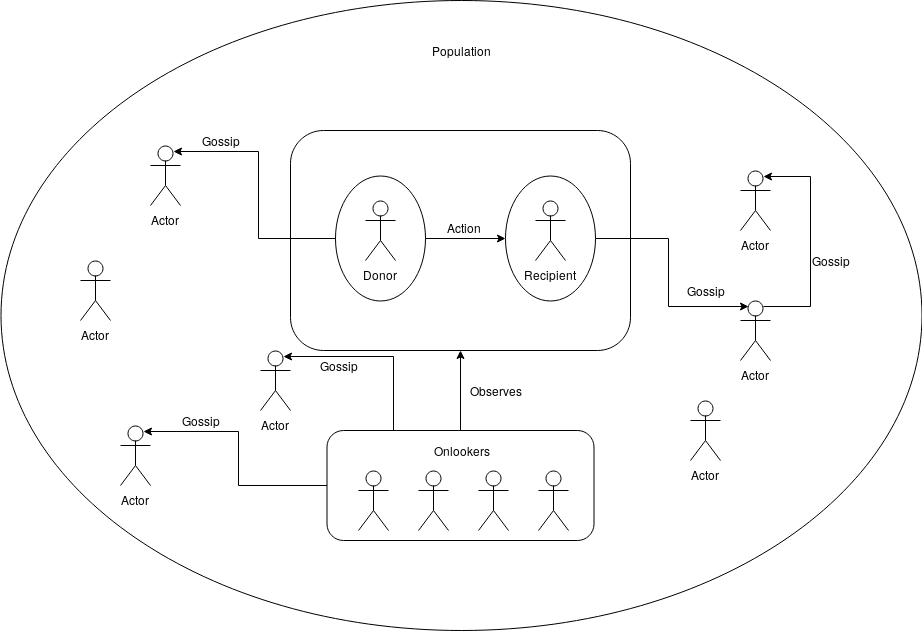
\includegraphics[width=0.5\textwidth]{Gossip_and_onlookers.png}
	\caption{The spread of information through a population using indirect reciprocity with gossip and onlookers}
	\label{fig:gossip_and_onlookers}
\end{figure}

\subsection{Comparison of Models}
The aim of Roberts~\cite{evoldirindir} is to compare the effectiveness of indirect reciprocity models and direct reciprocity. Roberts' results support Nowak and Sigmund's 1998 result that image scoring can support cooperation is robust even when criticisms relating to genetic drift and errors are taken into consideration.\\
However, it is highlighted that image scoring does not take into account who the donor is defecting against, whereas standing strategy does. Due to this image scoring suffers from an inability to distinguish between pure defectors and those who would cooperate with a cooperator. Standing strategy gives information both about how agents have interacted and the context of this action, an advantage over image scoring.\\
Counter to standing strategies perceived benefits it is seen that players are more susceptible to errors in perception, as standing falls faster than image score. Roberts also criticizes the standing strategy as not being a representation of the evolution of cooperation, as good standing can't have been established before the game had begun.\\
Roberts also points out that cooperation is only worth it when that cooperation is improving your chance of being cooperated with. This could be a counterpoint to the effectiveness of gossip as an alternative to direct observation. In gossip, there is a possibility of interactions being distorted by incorrect gossip. It could be interesting to see how the spread of misinformation could permeate society.

%------------------------------------------------

\section{A Concrete Model}
\subsection{Specification of the Model}
Both image scoring and standing strategy are good models for indirect reciprocity. They allow an agent to interpret a reputation and act as they see fit. However, the reputation of each player being universally viewable is unrealistic. The idea of onlookers seems closer to real life but is restrictive to the evolution of cooperation. The addition of gossip from these onlookers could be a sufficient alternative to direct observation, but gossip can be distorted by players wishing to influence proceedings against cooperation.\\
Gossip complicates a model because there is a need to interpret the information gossiped by another player. This also highlights an issue with the models that use purely standing strategy or image scoring: reputation is not a centralised system with everyone interpreting events the same way. Reputation has a very subjective nature, especially when gossip is introduced. Due to the subjectivity of perception about an agents reputation, I do not believe that one specific model for all agents can be considered appropriate. How a player views another players reputation must be up to their inside workings.\\
This requires an agent to have a view of past events and also a way to interpret these events in order to make decisions about another player. A model that uses this decentralised judgement on past events easily becomes a hybrid indirect and direct reciprocity game, as agents can have their own way to interpret interactions.\\
For an agent to interpret gossip, the gossip must be comprehensible by them and thus should have a given structure. In our model, gossip shall be split into two categories: positive and negative. Gossip will also involve 3 agents, the agent gossiping, the recipient of the gossip, and the gossip that the agent is about (who shall not be able to view that the gossip has taken place). Gossip is intended to change how the recipient of the gossip views the agent the gossip is about - for example, if agent 2 trusts gossip from agent 3 that is negative about agent 1 and agent 2 is using the standing strategy, then agent 2 will revise their beliefs about agent 1 to have a bad standing.\\
The structure of the game will be as follows. There is one singular population (this is to not overly complicate the model, though changing this to an island population model such as in Leimar and Hammerstein~\cite{leimarhammer}), a population is replaced by their offspring after the conclusion of a generation. A generation is made up of a number of interactions, all at a distinct time point (the number of interactions per generation is a variable).\\
In each time point, each agent will perceive their environment and then decide what action to take, this action may be as a donor in an interaction or maybe a piece of gossip. Each interaction shall be made up of a donor-recipient pair, chosen at random from the population. For each interaction, a subset of the population should be chosen as direct observers (being onlookers and the donor-recipient pair).\\
Finally, reproduction occurs at the end of every generation and will be relative to each players fitness. The fitness of a player represents how successful they are, fitness is altered in each interaction if the donor cooperates they lose a fitness point but the recipient gains two, if the donor defects they both gain nothing and lose nothing see table~\ref{tab:payoffmatrix}. Reproduction represents the replacement of agents with newer agents in a network. The new agents developed for a system would likely be influenced by successful strategies in past generations thus the reproduction in our system represents the trend towards certain successful strategies in a multi-agent system.\\
\begin{framed}
	\begin{center}
		\begin{tabular}{c|c|c}
		\multirow{2}{*}{Donor Action} & \multicolumn{2}{c}{Payoffs}\\		
		& Donor & Recipient\\
		\hline
		Cooperation & -1 & 2\\
		\hline
		Defection & 0 & 0\\
		\end{tabular}
		\captionof{table}{The payoff for my indirect reciprocity model}
		\label{tab:payoffmatrix}
	\end{center}	
\end{framed}
The group size remains the same over generations in order to measure the success of different strategies in certain group sizes, so in a new generation individuals are generated and assigned strategies. The chance an individual will be a certain strategy is worked out by summing the fitness of all individuals of that strategy and dividing it by the fitness of the overall group. Reproduction in this way has been chosen to represent the way that new agents will tend to be developed based on past successful strategies. The user will be able to select if mutation is active or not, if it is there will be a 1\% chance that a new individuals strategy will be chosen completely at random.

\subsection{Specification of Agent Strategies}
At each time point in the generation that an agent is a part of, the agent may perceive new information about interactions and gossip that has occurred in the game by way of an environment sending new percepts to agents. The agent will then be asked to decide on what they want to do at that same time point.\\
The percepts that the agent can receive is that they are a donor at this time point, that they are a recipient at this time point, gossip from another agent and observation of an interaction at the last time point.\\
Based on the percepts an agent will be able to revise their beliefs about other agents and the environment. For all agents, if they perceive that they are a donor in a donor-recipient pair they revise their beliefs to know that they are a donor at this time point. However, the revision of beliefs is generally strategy dependent, for example, in an agent using the standing strategy if they observe an interaction where a donor defects against an agent that you consider to have good standing the observing agent will revise their beliefs to give a bad standing to the donor.\\
Agents will have a theory on the best action to take based on their beliefs, if they have not yet received percepts they may not have any beliefs yet, so will have to have a default action. Based on the agents' beliefs and strategy they will have a theory encoded on how is best to act at each time point. The theory encoded is dependent on the strategy they are using, for example, if a discriminator (with k=2) has perceived they are a donor and that the recipient of their action has an image score of 1 the theory will say it is best to defect, as the image score is lower than their value of k. It will also be important to encode a theory on how to act if an agent is not a donor (how do they spread gossip? Do they remain idle?).\\
Of course, some agents will not care about percepts on other agents and will purely decide according to a plan such as always defect, or always cooperate. However, there needs to be a distinction on how an agent reacts to gossip and how they react to an observation. I propose two classes of interpretation: trusting and distrusting. Distrusting agents will never take into account gossip, however, trusting agents will have a trust model, for example trusting agents using the standing strategy will only believe gossip and allow it to change their view of another agent's standing if the agent gossiping to them has a good standing from their point of view. Another example of this is if an agent is using a distrusting standing strategy, negative gossip will not change their beliefs on the standing of a certain agent.\\
Using this design, strategies that will be implemented include: trusting and distrusting `neutral' standing discriminator (similar to Roberts' version), trusting and distrusting image scoring discriminator (with varying values of k), cooperator, defector. This is not an exhaustive list and I will be including more strategies based on `neutral' standing and image scoring.\\
These strategies only describe how to act as a donor based on beliefs on another agent. An agent will also need a strategy of how to act when it is not a donor. Some strategies may include: stay idle, always gossip accurate information to random players (if none then stay idle), always gossip inaccurate information to random people, always gossip negative or positive information to random players, randomly gossip positively or negatively. More advanced agents will have a better-developed strategy for when they are not a donor.\\
In conclusion, basic agents will need a way to take in percepts, they will then need a strategy to act if they are a donor and if they are not a donor. More advanced agents will use percepts to revise their beliefs and then use their beliefs to decide on how to act at any given time point. Even more advanced agents than these will develop beliefs or act on beliefs in more interesting ways than discriminating based on their view of whether an agent has a good standing or whether their view of an agents image score is above a certain value. Examples of these more advanced strategies are: basing their action on both their own and the recipients standing or image score or using a reinforcement algorithm to decide an action based on a belief.


%------------------------------------------------

\section{Discussion and Conclusion}
Multi-agent systems require agents to be autonomous, they should not be working on centralised beliefs such as is used by Nowak and Sigmund~\cite{evol_indirect_image} at first. My model not only removes those centralised beliefs and makes them part of the agent's inner workings but also makes the whole strategy they use part of the agent's inner workings. \\
The lack of individuality is where the work on indirect reciprocity I have seen falls short, because of the nature of indirect reciprocity being a community-driven mechanism the implementors see beliefs as community held and fail to realise that the beliefs may be community driven, but are actually individually held.\\
This model is also very open to extension. Extensions on the population model (maybe using the island idea), the strategies (different interpretations of gossip and observations, strategies for the spread of gossip and strategies for actions as a donor) and mixing in indirect reciprocity by viewing observations where the agent is a recipient differently.



%----------------------------------------------------------------------------------------
%	REFERENCE LIST
%----------------------------------------------------------------------------------------

\bibliography{../refs.bib}{}
\bibliographystyle{plain}

%----------------------------------------------------------------------------------------

\end{document}
